\newpage
\section{Zasada działania programu}
Przydzielona metoda symulacyjna to \textbf{metoda przeglądania zdarzeń (M1)}. W tej metodzie, w każdym obrocie pętli głównej programu, wyszukiwane jest zdarzenie (ang. \emph{event}), którego znacznik czasowy jest najmniejszy. Następnie licznik czasu symulacji ustawiany jest na tą wartość i wykonywane jest zdarzenie. Po wykonaniu zdarzenia czasowego program sprawdza czy zostały spełnione warunki zdefiniowane dla zdarzeń warunkowych i gdy jest to wymagane, również wykonuje te zdarzenia. 
\newline\newline
\noindent Zidentyfikowane zdarzenia czasowe w zadaniu to:
\begin{itemize}
\item Pojawienie się nowego użytkownika w stacji bazowej -- \emph{AddUser}
\item Zakończenie obsługi użytkownika -- \emph{ReleaseUser}
\item Zakończenie przejścia stacji ze stanu aktywnego do stanu uśpienia -- \emph{ShutDown}
\item Zakończenie przejścia stacji ze stanu uśpienia do stanu aktywnego -- \emph{PowerUp}
\end{itemize}

\noindent Zidentyfikowane zdarzenia warunkowe w zadaniu to:
\begin{itemize}
\item Przekierowanie użytkownika z pełnej stacji bazowej do innej
\item Rozpoczęcie przełączania stacji aktywnej w tryb uśpienia, gdy jej zużycie zasobów jest poniżej odpowiedniego progu
\item Rozpoczęcie przełączania stacji uśpionej w tryb aktywny, gdy zużycie zasobów stacji aktywnej jest powyżej odpowiedniego progu
\end{itemize}

\noindent Działanie pętli głównej symulacji zostało przedstawione na rysunku \ref{main_loop}. W pierwszej kolejności tworzona jest instancja struktury \emph{SimState}, zawierającej stan symulacji. Następnie, tak długo jak znacznik czasu stanu symulacji jest mniejszy od całkowitego czasu trwania z konfiguracji, wykonywana jest pętla główna, na którą składają się poniższe czynności:
\begin{enumerate}
\item Aktualizacja wartości $\lambda$ -- następuje gdy aktualny czas symulacji jest większy od, zapisanego w stanie symulacji, czasu aktualizacji wartości $\lambda$. Wartość \emph{lambda} z konfiguracji jest mnożona przez kolejny współczynnik z listy \emph{lambda\_coefs} oraz obliczany jest czas kolejnej aktualizacji. Obsługa tego zdarzenia została rozdzielona od obsługi zdarzeń pochodzących ze stacji bazowych, aby poprawić czytelność i wydajność programu
\item Wybór najbliższego zdarzenia -- każda stacja bazowa jest odpytywana o najbliższe zdarzenie, z których wybierane jest jedno, o najmniejszym znaczniku czasu, i zapisywane w tymczasowej zmiennej. Czas symulacji jest ustawiany na wartość znacznika czasu wybranego zdarzenia
\item Wykonanie zdarzenia -- Zapisane zdarzenie jest przekazywane do odpowiedniej stacji do obsługi. Pełna procedura została przedstawiona na rysunku \ref{station_event}. Użytkownik zostanie dodany do stacji tylko gdy jest ona aktywna oraz posiada wolne bloki zasobów. W każdym innym przypadku użytkownik zostanie zwrócony do systemu. W przypadku zdarzenia zakończenia obsługi użytkownika, jeżeli wszystkie bloki zasobów stacji są wolne, zostanie to uznane za krytyczny błąd i nastąpi przerwanie wykonywania programu
\item Obsługa przekierowania -- jeżeli zdarzeniem było pojawienie się nowego użytkownika, a stacja bazowa zwróciła go do systemu w celu przekierowania, wybierana jest stacja z najmniejszym zużyciem zasobów w systemie. Jeżeli wybrana stacja ma wolny blok zasobów, użytkownik jest przypisywany do tej stacji. W przeciwnym razie użytkownik jest tracony
\item Sprawdzenie możliwości uśpienia/ wybudzenia stacji -- następuje gdy użyty jest przełącznik \emph{-{}-enable-sleep}. Jeżeli zużycie zasobów dowolnej stacji w systemie przekracza odpowiedni próg z konfiguracji, następuje próba wybudzenia jednej z uśpionych stacji i przekazania jej połowy użytkowników. W przeciwnym wypadku wyszukiwana jest stacja, której zużycie zasobów jest poniżej drugiego progu z konfiguracji. Jeżeli taka stacja została znaleziona, następuje próba przełączenia jej w stan uśpienia. Pełna procedura została pokazana na rysunku \ref{power_up_down}
\end{enumerate}

\noindent Aby przyspieszyć działanie programu, wszystkie iteracje są wykonywane równolegle, za pomocą iteratorów z biblioteki \emph{Rayon}. Z tego powodu przebiegi symulacji są niezależne względem siebie i wszystkie zasoby, niezbędne do jej wykonania, są tworzone indywidualnie dla każdego przebiegu.


\begin{figure}
\center
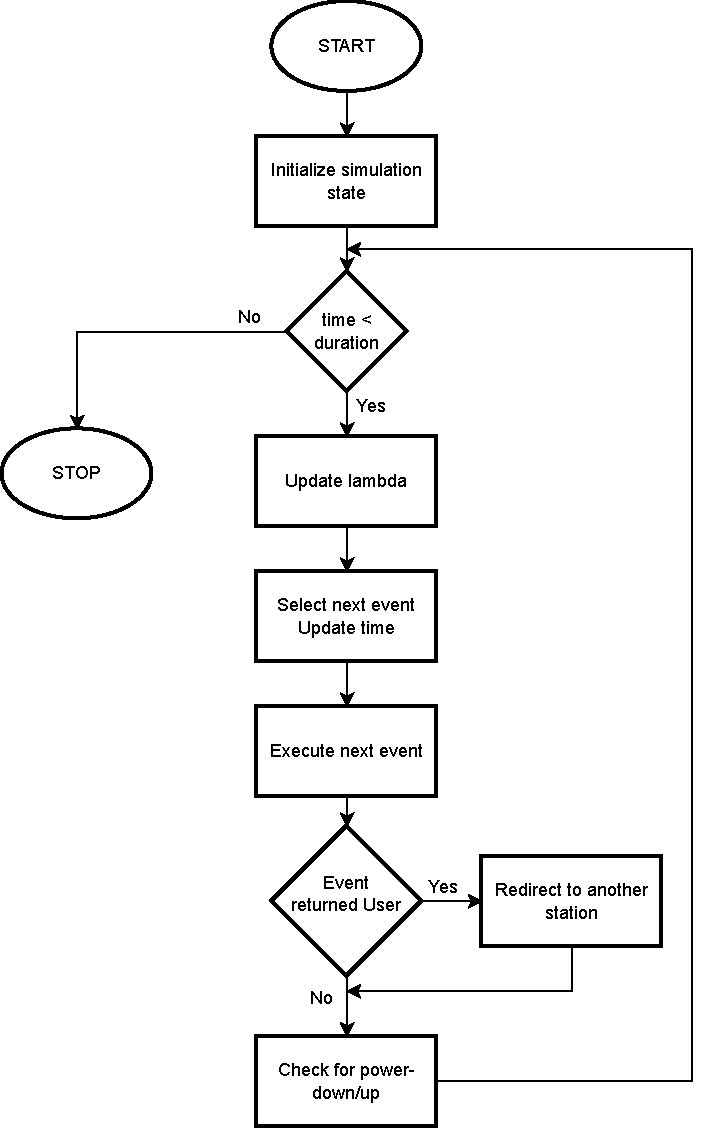
\includegraphics[scale=0.78]{img/main_loop.pdf} 
\caption{Schemat blokowy pętli głównej programu}
\label{main_loop}
\end{figure}

\begin{figure}
\center
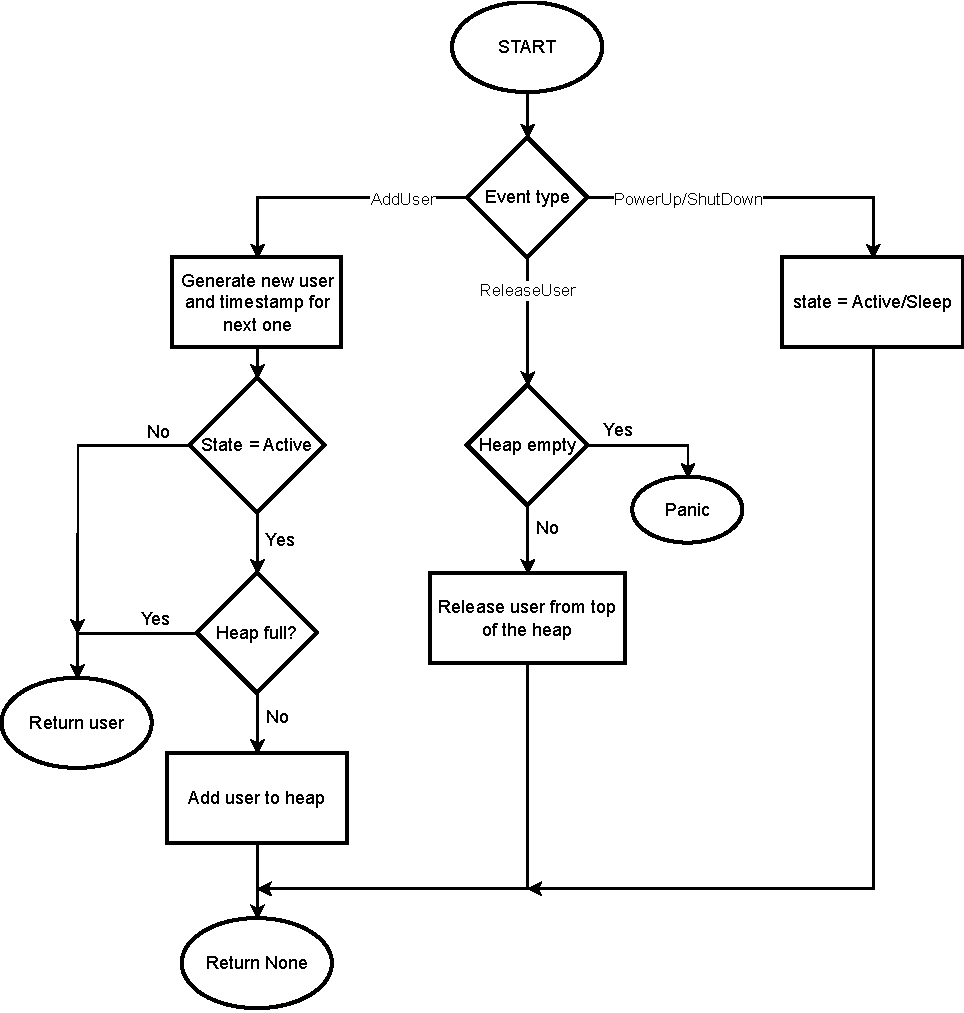
\includegraphics[scale=0.8]{img/station_event.pdf} 
\caption{Schemat blokowy pętli głównej programu}
\label{station_event}
\end{figure}


\begin{figure}
\center
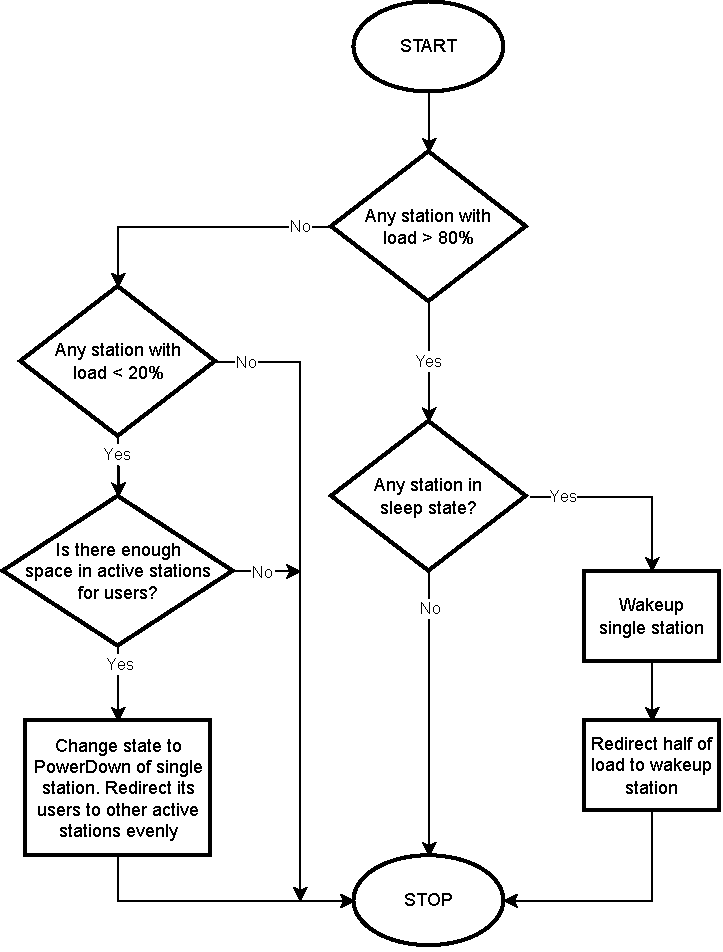
\includegraphics[scale=0.8]{img/power_up_down_logic.pdf} 
\caption{Schemat blokowy pętli głównej programu}
\label{power_up_down}
\end{figure}